\documentclass{standalone}
\usepackage{tikz}
\usetikzlibrary{positioning,calc}

\begin{document}
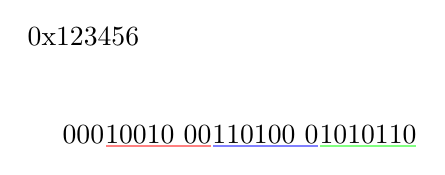
\begin{tikzpicture}[every node/.style={inner sep=0pt}]
  \node at (0,0)    (0) {0x123456};
  \node[below=of 0] (1) {000};
  \node[anchor=west,right=0pt of 1.east] (2) {10010 00};
  \node[anchor=west,right=0pt of 2.east] (3) {110100 0};
  \node[anchor=west,right=0pt of 3.east] (4) {1010110};
  \draw[thick,red!50] ($(2.south west)+(.5pt,-.8pt)$) -- ($(2.south east)+(-.5pt,-.8pt)$);
  \draw[thick,blue!50] ($(3.south west)+(.5pt,-.8pt)$) -- ($(3.south east)+(-.5pt,-.8pt)$);
  \draw[thick,green!50] ($(4.south west)+(.5pt,-.8pt)$) -- ($(4.south east)+(-.5pt,-.8pt)$);
\end{tikzpicture}
\end{document}